\section{MTConnect}

\subsection{What is MTConnect?}

MTConnect is an open and royalty-free set of standards designed as a universal factory floor communications protocol. MTConnect is intended specifically for the shop floor environment. While there are numerous communication solutions available, MTConnect defines a “dictionary” for manufacturing data. This means that all data is provided with full context – name, definition, scaling, etc. With most communication networks, all data is defined at the point of use – the application. With MTConnect, the data is defined at the source – the device or Machine Tool. MTConnect devices process information locally and then provide that data in a consistent format to any client application requesting data - ERP, MES, Production Management Systems, Maintenance Systems or a standard Browser, for examples.

\subsection{Basics of MTConnect}

MTConnect is based on standard Internet technologies – HTTP, Ethernet, and XML (Extensible Mark-Up Language – the underlying language of most web sites).
As an Extensible Standard, MTConnect cannot address every conceivable data need on the shop floor. MTConnect provides a clearly defined method for adding additional data types which can be exchanged between equipment, devices, controllers and applications; providing the flexibility to meet the demands of varying environments. 

MTConnect is made up of five fundamental components (see Figure \ref{fig:mtconnect_overview} below):
\begin{itemize}
\item \textbf{Device} -- A type of equipment (Machine Tool) or data source.
\item \textbf{Adapter} -- An optional piece of software (and sometimes hardware) that provides a link or conversion from the data source and data definition in the device to the MTConnect Data definition.  This can be thought of as a translator. The Adapter is not needed for devices that use MTConnect as their native language.
\item \textbf{Agent} -- A piece of software that collects, arranges, and stores data from the device.  It receives requests for data from applications, processes those requests, and then transmits the required data.
\item \textbf{Network} -- The physical connection between a data source (device) and the data consumer (application).  Normally, this is an Ethernet network. The communication on the network normally uses standard internet communications methods – http:// protocol. It should be noted that the MTConnect Structure is adaptable and can be implemented in conjunction with other networking solutions other than Ethernet and Internet protocols.
\item \textbf{Client} -- A Client initiates all requests for MTConnect data. A Client resides in an application or device. The Client is a software function in the application or device that actually requests data from the Agent. 
\end{itemize}

\begin{figure}[h]
  \centering
  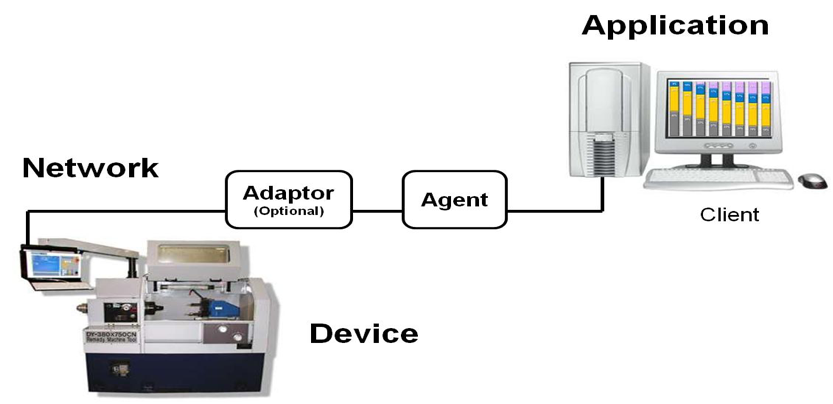
\includegraphics[width=0.75\textwidth]{diagrams/MTConnectOverview.png}
  \caption{MTConnect Overview}
  \label{fig:mtconnect_overview}
\end{figure}

The MTConnect Standard does not restrict the physical implementation of how the MTConnect system is designed.

\begin{itemize}
\item The Network may be a physical implementation, like an Ethernet network. It can also be implemented using wireless or other technologies.
\item The Internet Protocol (http) does not mean that your machine is automatically connected outside your plant to the Internet. This is a communications method only. Protection of your data is controlled by your networking standards. 
\item There is no specific requirement for where the Adapter and Agent function is located. These can be located at the device. However, they can be placed anywhere in the networking architecture. Also, they do not need to be located together. MTConnect can to have the Adapter installed at the device and the Agent installed along with the Client. The location of these functions should be considered when implementing MTConnect since they will impact the level of data flow on different segments of your network.
\end{itemize}
